%
% LaTeX template for Dual Degree / Masters thesis at IITB
%
% Created by Neehar Jathar
%
% The official requirement has been persisted with, even if some things could look better some other way.
% Tamper with any of the settings as you see fit and, more importantly, as your guide sees fit.
% Most sections have comments. A lot of stuff is explained in Chapter 1 regarding how to use this template.
% Code snippets for inserting figures, tables and equations are also there in Chapter 1
% Hopefully, this will make report making a little easier.
%

% OK. Here goes.

% Preamble

% Official font size is 12. I thought 11 looked better.
% A4 paper size
% Template for one sided printing of the thesis
\documentclass[12pt, a4paper, oneside]{book}

% Set of packages included. These are all the packages I required, maybe some would be unnecessary and some might be missing. 
% Add any new packages you use over here.

\usepackage[utf8]{inputenc}
\usepackage{setspace}
\usepackage{amsmath,amsfonts,amssymb,amscd,amsthm,xspace}
\usepackage{titlesec}
\usepackage{vmargin}
\usepackage{fancyhdr}
\usepackage{caption}
\usepackage{subcaption}
\usepackage{multirow}
\usepackage{multicol}
\usepackage{url}
\usepackage{tabularx}
\usepackage{graphicx}
\usepackage{epstopdf}
\usepackage{booktabs}
\usepackage{rotating}
\usepackage{listings}
\usepackage{algpseudocode}
\usepackage{algorithm}

%% for algorithmic package %%
%\floatname{algorithm}{Procedure}
\renewcommand{\algorithmicrequire}{\textbf{Input:}}
\renewcommand{\algorithmicensure}{\textbf{Output:}}
%%          end            %%

%\usepackage[centerlast,small,sc]{caption}
\usepackage[square, numbers, comma, sort&compress]{natbib} % Standard reference style with [3], [4] type numbers in the text and entries sorted according to order of appearance in the References
\usepackage[pdfpagemode={UseOutlines},bookmarks=true,bookmarksopen=true,bookmarksopenlevel=0,bookmarksnumbered=true,hypertexnames=false,colorlinks,linkcolor={black},citecolor={black},urlcolor={black},pdfstartview={FitV},unicode,breaklinks=true]{hyperref}
\hypersetup{urlcolor=black, colorlinks=true} % colors hyperlinks in blue - change to black if annoying

% Math operator definition - may not be required
% If any new operators are required, defien them here
\DeclareMathOperator*{\argmin}{argmin}

\title{\thesisTitle}
\author{\authorName}
\date{\today}

% Currently chapter title has been centered, to left align the chapter title and number, change \centering to \flushleft
\titleformat{\chapter}[display]
  {\normalfont\huge\bfseries\centering}
  {\chaptertitlename\ \thechapter}{18pt}{\Huge}

\setmarginsrb   { 3.0cm}  % left margin
                { 1.5cm}  % top margin
                { 2.0cm}  % right margin
                { 2.2cm}  % bottom margin
                { 0.3cm}  % head height
                { 1.2cm}  % head sep
                { 0.3pt}  % foot height
                { 1.0cm}  % foot sep

% End of the Preamble

% Actual document begins
\begin{document}

\newcommand{\HRule}{\rule{\linewidth}{0.5mm}} % New command to make the lines in the title page

% Import all the variable values from Details.tex
% This file contains all the user specific things that need to be changed such as the thesis title, author name etc. 


\newcommand{\thesisTitle}{Implementation of a Parallel SAT Solver}

\newcommand{\degree}{Bachelor of Technology and Master of Technology}

\newcommand{\authorName}{Sahil Agarwal}

\newcommand{\rollNo}{10D070017}

\newcommand{\dept}{Department of Electrical Engineering}

\newcommand{\college}{Indian Institute of Technology Bombay}

\newcommand{\currentyear}{2014}

\newcommand{\currentmonth}{October}

\newcommand{\supervisorOne}{Prof. Madhav Desai}

\newcommand{\supervisorTwo}{Prof. Supervisor Two}

\newcommand{\examinerOne}{Prof. Examiner One}

\newcommand{\examinerTwo}{Prof. Examiner Two}

\newcommand{\chairman}{Prof. Chairman}


% Use roman page numbering style (i, ii, iii, iv...) for the pre-content pages
\frontmatter

% Line spacing of 1.5 as per IIT requirement. If you think it looks too spaced out, use 1.3
% I think 11 pt font with 1.3 spacing looks quite good
\setstretch{1.5}

% Import all the pages in the front matter
% This file contains the templates for the first few pages of the thesis including 
% 1. Title page
% 2. Dedication
% 3. Dissertation approval
% 4. Declaration of authorship
% 5. Abstract


%   1. TITLE
\newcommand{\titlePage}{

% No page number
\thispagestyle{empty}
\begin{center}

% thesis title
\vspace*{15px}
{\Huge\bfseries \thesisTitle}\\[1.0cm] 

% submitted in partial fulfillment etc.
\textit{Submitted in partial fulfillment of the requirements\\[0.2cm] of the degree of\\[0.2cm] \degree}\\[1.5cm]
 
% author
\textit{by}\\[0.2cm]
\authorName \\[0.2cm] (\textit{Roll no.} \rollNo) \\[1.5cm]

% supervisor
\textit{Supervisor:}\\[0.2cm]
% or
% \textit{under the supervision of}\\[0.2cm]
\supervisorOne \\[2.0cm]

% iit-b logo

\includegraphics[width=0.25\textwidth]{Figures/iitb_logo.jpg}

\vspace*{10px}

% department and college
\dept\\[0.2cm]
\college\\[0.2cm]

% year
\currentyear\\[4cm] 

\end{center}

\clearpage
}

%   2. DEDICATION
\newcommand{\dedication}{
\thispagestyle{empty}
\vspace*{75px}
\begin{center}\large{\textit{Dedicated to ...}}\end{center}

\clearpage
}

%   3. DISSERTATION APPROVAL

\newcommand{\approval}{
% if you use a dedication, then use a page number with the plain page style
\thispagestyle{plain}
% else, use no page number with the empty page style
%\thispagestyle{empty}


% page title
\begin{center}{\huge\bf Dissertation Approval\par}\end{center}

\vspace*{15px}

\noindent This dissertation entitled 
% title
\textbf{``\thesisTitle"}, submitted by 
% author
\authorName  
(Roll No.  \rollNo),
is approved for the award of degree of 
% degree
\degree 
in 
% branch
XYZ Engineering.\\[1.0cm]

% examiners and supervisors
\begin{flushright}
\textbf{{Examiners}}\\[0.8cm]
\examinerOne\quad\rule{0.3\textwidth}{.3pt}\\[0.8cm]
\examinerTwo\quad\rule{0.3\textwidth}{.3pt}\\[1.6cm]

\textbf{{Supervisor}}\\[0.8cm]
\supervisorOne \quad\rule{0.3\textwidth}{.3pt}\\[1.6cm]

\textbf{{Chairman}}\\[0.8cm]
\chairman\quad\rule{0.3\textwidth}{.3pt}\\[2.4cm]

\end{flushright}
\textbf{Date:} ...... \currentmonth { } \currentyear\\[0.3cm]
\textbf{Place:}\quad\rule{0.5\textwidth}{.3pt} 

% start a new page
\clearpage
}

%   4. DECLARATION OF AUTHORSHIP
\newcommand{\authorship}{
\thispagestyle{plain}

\begin{center}{\huge\bf Declaration of Authorship\par}\end{center}

\vspace*{15px}

% institute declaration text
\noindent I declare that this written submission represents my ideas in my own words and where others' ideas or words have been included, I have adequately cited and referenced the original sources.  I also declare that I have adhered to all principles of academic honesty and integrity and   have   not   misrepresented   or   fabricated   or   falsified   any   idea/data/fact/source   in   my submission.  I understand that any violation of the above will be cause for disciplinary action by the Institute and can also evoke  penal action from the sources which have thus not been properly cited or from whom proper permission has not been taken when needed.

\vspace*{10px}

% signature
\begin{flushright}
{Signature: ......................................\\[0.4cm]}

% author name
{\textbf{\authorName}\\[0.0cm]\rollNo\\[2.0cm]}

\end{flushright}
% date
\begin{flushleft}
{Date: ...... \currentmonth { } \currentyear\\}
\end{flushleft}


% start a new page
\clearpage 
}

%   5. ABSTRACT
\newcommand{\abstractpage}{
\thispagestyle{plain}

% header-type text for the abstract - optional
%\small {\noindent\authorName/ \supervisorOne{ }(Supervisor): \textbf{``\thesisTitle"}, \textit{Dual Degree Dissertation}, \dept, \college, \currentmonth { } \currentyear.}\\[0.0cm]
%\HRule\\[0.2cm]


\vspace*{10px}

\begin{center}{\huge{\textit {Abstract}}\par}\end{center}

\vspace*{10px}

% Abstract text - Type abstract here
\noindent SAT solvers are used in various domains like artificial intelligence, circuit design, automatic theorem proving, etc. With increasingly large search spaces, greater speed in solving is required. Modern SAT solvers are using available multi-core systems to achieve speedup in SAT solving. In this work we present a parallel SAT solver based on Orthonormal function decomposition \cite{sule14}. The solver will be implemented on clusters of computers, using OpenMP and MPI (Message Passing Interface). The main features of the program are described. The solver could also be used to solve other NP-hard problems like Travelling Salesman problem, Discrete Logarithm problem and more. 
 \\[0.2cm]

% Index terms
%\noindent \textbf{Index terms:} 

% Start a new page
\clearpage 
}


\titlePage

\setcounter{page}{1}
%\dedication

%\addcontentsline{toc}{chapter}{Dissertation Approval}
%\approval

%\addcontentsline{toc}{chapter}{Declaration of Authorship}
%\authorship

\addcontentsline{toc}{chapter}{Abstract}
\abstractpage

\pagestyle{fancy}

% Set the left side page header to "Contents"
\lhead{\emph{Contents}} 

% Write out the Table of Contents
\tableofcontents 

% Set the left side page header to "List of Figures"
%\lhead{\emph{List of Figures}} 

% Write out the List of Figures
%\listoffigures 
%\addcontentsline{toc}{chapter}{List of Figures}

% Set the left side page header to "List of Tables"
%\lhead{\emph{List of Tables}} 

% Write out the List of Tables
%\listoftables
%\addcontentsline{toc}{chapter}{List of Tables}

\fancyhead{}
\rhead{\thepage}


% Use arabic page numbering style (1, 2, 3...) for the body of the report
\mainmatter

% Import the Chapters
%% Introduction

% Main chapter title
\chapter{Introduction} 

% Change X to a consecutive number; for referencing this chapter elsewhere, use \ref{ChapterX}
\label{Chapter1} 

% This is for the header on each page
%\lhead{Chapter 1. \emph{Introduction}}  

This is a super quick tutorial on how to use this \LaTeX
template. The template has been made keeping the guidelines given by IIT in mind almost to the letter. The guidelines page is also included in the folder.

% SECTION 1
\section{Document Structure}

The folder contains the following files - 
\begin{enumerate}
\item \textit{main.tex} - This is the file to be compiled, as any self respecting main should be. It contains a bunch of settings which are (hopefully) adequately explained.
\item \textit{TheFrontMatter.tex} - This contains details about the first few pages including the title page, approval page, declaration of authorship, abstract etc.
\item \textit{TheBackMatter.tex} - This contains details about the list of publications page and the acknowledgements page.
\item \textit{Details.tex} - Enter all details such as thesis title, your name, supervisor's name, department etc. in this file. It will be substituted throughout the document.
\item \textit{ChapterTemplate.tex} - Use this as a template to generate more chapter files as and when required. Number them in order and then include them in main where mentioned
\item \textit{Chapter1.tex} - This is a README on how to use this template.
\item \textit{AppendixTemplate.tex} - If you need Appendices, works the same as the Chapter template.
\end{enumerate}

\section{Inserting Stuff}

The syntax for inserting figures, tables and equations can be picked up from the file Chapter1.tex.

\subsection{Figures}

\begin{figure}
\centering
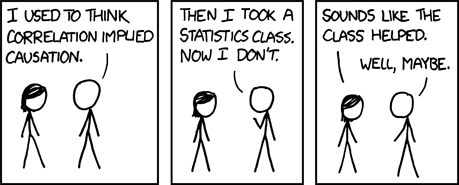
\includegraphics[width=0.8\textwidth]{Figures/xkcd.png}
\caption[Text that you want on the list of figures page]{Text that you want below the figure}
\label{fig:nameForThisFigure}
\end{figure}

Refer to figures using - \begin{verbatim}\ref{label} \end{verbatim} For example, this is how you can refer to Figure \ref{fig:nameForThisFigure}, no need to keep track of the numbers. Save all images in the Figures folder in .png or .jpg format. This image has been taken from \citep{xkcd}.

\subsection{Tables}

\begin{table}
\centering
\caption[Text that you want on the list of tables page]{Caption which will appear above the table}

\begin{tabular}{c|c|c|c}
Header1 & Header 2 & Header 3 & Header 4 \\ \hline
data & data & data & data \\
data & data & data & data \\ \hline
\end{tabular}

\label{tab:nameForThisTable}
\end{table}
 
This is how you can refer to Table \ref{tab:nameForThisTable}.

\subsection{Equations}

\begin{equation}
X = \sum_{i=1}^{N}{\frac{i+1}{i^2 + 3\alpha\beta_0}}
\label{eqn: equationLabel}
\end{equation}

Equations also number themselves and can be referred in the same way as tables and figures.

\section{Dealing with References}

Find the paper you need on Google Scholar. Click on Cite. Click on Import into BiBTeX. Copy the text into Bibliography.bib. The first entry is the reference label. Use that label to refer to the paper anywhere in the document using - 
\begin{verbatim}
\citep{label}
\end{verbatim}





\chapter{Introduction}

\section{Boolean Satisfiability Problem}

The Boolean Satisfiability Problem (SAT) is the problem of determining if there exists an interpretation that satisfies a given Boolean formula. An interpretation is the assignment of TRUE or FALSE values to variables of the given formula. If an assignment exists such that the formula evaluates to TRUE, the formula is called satisfiable. If no such assignment exists, the function expressed by the formula is identically FALSE for all possible variable assignments and the formula is unsatisfiable. A \textit{SAT solver} is the algorithm which solves the SAT problem.

\textbf{Definitions and Terminology:} A propositional logic formula, also called Boolean expression, is built from variables, operators AND (conjunction, also denoted by $\wedge$), OR (disjunction, $\vee$), NOT (negation, $\neg$), and parentheses. A literal consists of a variable A and is either positive ($A$) or negated
($\neg A$). A clause is a disjunction of literals. A formula is in the conjunctive normal form (CNF) if it is a conjunction of clauses. A boolean formula is generally given to the SAT solver in CNF.

\section{Overview of SAT solvers} 

\subsection{DPLL Algorithm}

Most modern SAT-solvers are based on
the Davis-Putnam-Loveland-Logemann (DPLL) algorithm \cite{DPLL}. It is a complete, backtracking-based search algorithm for solving the CNF-SAT problem. \footnote{Henceforth, the input formula is in CNF unless specified otherwise.}

The \textit{backtracking algorithm} runs by choosing a literal, assigning a truth value to it, simplifying the formula and then recursively checking if the simplified formula is satisfiable; if this is the case, the original formula is satisfiable; otherwise, the same recursive check is done assuming the opposite truth value. This is known as the \textit{splitting rule}, as it splits the problem into two simpler sub-problems.

The DPLL algorithm enhances over the backtracking algorithm by using the following rules at each step:
\begin{itemize}
\item \textit{Unit propagation} - If a clause is a unit clause, i.e. it contains only a single unassigned literal, this clause can only be satisfied by assigning the necessary value to make this literal true.

\item \textit{Pure literal elimination} - If a propositional variable occurs with only one polarity in the formula, it is called pure. Pure literals can always be assigned in a way that makes all clauses containing them true. Thus, these clauses do not constrain the search anymore and can be deleted.
\end{itemize}

Unsatisfiability of a given partial assignment is detected if one clause becomes empty, i.e. if all its variables have been assigned in a way that makes the corresponding literals false. This is known as the \textit{conflict clause}. Satisfiability of the formula is detected either when all variables are assigned without generating the empty clause, or, in modern implementations, if all clauses are satisfied. Unsatisfiability of the complete formula can only be detected after exhaustive search.

\subsection{Sequential SAT solvers}
The idea to analyze the conflict clause further led
to the conflict driven clause learning (CDCL) \cite{GRASP}. Resolving the conflict clause and the
clauses which have been used in the implications, new
clauses are learned. These learned clauses can be added
to the given formula leading to an improved backtracking
behavior, where larger parts of the search tree are
closed by a single conflict. The most commonly used
version of this algorithm is described in \cite{cdcl}.

The most commonly used SAT-solver that implements
most of the mentioned techniques is MINISAT (\cite{minisat}). This solver provides a basis for many sequential and parallel SAT-solvers including the one implemented in this work.

\subsection{Parallel SAT solvers}

The recursive application of the split rule in the
DPLL algorithm provides a natural way to parallelize
the search for a satisfying assignment \cite{overview}. Initially, each computing node receives
the given formula. Thereafter, only partial interpretations
are communicated such that each computing
node receives a different partial interpretation. This is the \textit{Decomposition-based approach}. The
first parallel SAT-solvers used single-core CPUs which
communicated via a network. When shared memory
architectures became available, shared memory communication
was utilized. A popular decomposition-based parallel solver is PMSAT \cite{pmsat}. It is based on MiniSAT 1.14 and MPI (Message Passing Interface).


Another popular technique in parallel SAT solving is the \textit{Portfolio-based technique}. Instead of implementing cooperative parallelism by splitting the
search space, competitive parallelism is applied where all parallel
solvers try to find a solution for the same SAT instance. 

\section{A new parallel SAT solver}

\subsection{High-level description}
This work highlights a decomposition-based parallel SAT solving algorithm. The algorithm is based on the application of a well
known generalized Boole-Shannon orthonormal (ON) expansion of Boolean functions \cite{sule14}. This is basically an extension of the DPLL algorithm in which the splitting rule is generalized to several variables in terms of ON terms. The subproblems created recursively are solved on parallel computing nodes. After a threshold is reached, direct sequential search is performed on the subproblems at the individual nodes.

\subsection{Motivation}
Until now, modern CPUs contain only few cores.
Recent parallel SAT-solvers for such shared-memory
architectures are mainly based on the techniques developed
for sequential SAT-solvers. As soon as the individual
solvers running on different cores share memory,
the efficiency of the individual solvers decreases. None
of these parallel solvers seem to scale well if hundreds
or even thousands of cores become available. 

The algorithm suggested above has the potential to make use of large number of cores due to ease in its parallelization.

\chapter{Implementation of the SAT solver}

\section{Introduction}

The parallel SAT solver will use the Orthonormal (ON) expansion based algorithm in \cite{sule14}. This algorithm is a generalized version of the DPLL algorithm \cite{DPLL}.

\section{Plan}
\begin{itemize}
\item \textit{Sequential Stage} - A sequential form of the algorithm has been implemented in the first stage. Although this will not give an idea of execution time of the parallel algorithm, it can be used to verify the correctness of the approach.

\item \textit{Parallel Stage 1} - The algorithm will undergo slight modifications to achieve parallelism using OpenMP (Open Multi-Processing). OpenMP is an API that supports multi-platform shared memory multiprocessing programming in C, C++ \ldots \cite{openmp}. This is a single machine multi-core implementation. 

\item \textit{Parallel Stage 2} - Large-scale parallelization over multiple machines and cores will be achieved by using MPI (Message Passing Interface). MPI was also used in \cite{pmsat}.
\end{itemize}
\section{Implementation}




\textbf{Class} \textit{Solver} - It is the basis of the entire solver. It contains the data structure $C$ which stores the clauses. Its member functions help interect with the class and can be used to solve SAT problems.

Below is the description of the important components of the solver:

\begin{itemize}

\item \textit{Main}() (Algorithm \ref{main}) takes as input the CNF file and stores the clauses in C. Calls Solve() and outputs SAT/UNSAT.

\item $C$ - It refers to the data structure which stores the clauses using \textit{sparse matrix representation}.

\item \textit{Solver::Solve}() (Algorithm \ref{algo}) is called by the main program. It takes as input $C$ and $n_0$. It decides whether to decompose further or solve by direct search over all assignments. It returns whether the input problem is SAT or UNSAT.

\item \textit{Solver::Decompose}() (Algorithms \ref{decompose} and \ref{dist}) decides an ON set of terms and decomposes the input problem. It calls \textit{Solve}() for each of the reduced problems.

\item \textit{Solver::Simplify}() consists of functions \textit{unitpropagate}() and \textit{pureliterals}() which simplify the problem and remove satisfied clauses.

\item \textit{Solver::SolveMinisat}() is a function that takes as input $C$ and returns SAT/UNSAT. It uses the Minisat solver \cite{minisat}.
\end{itemize}

The sequential algorithm uses Algorithms \ref{algo} and \ref{decompose}. The parallel implementation will only need a slight modification in the decompose() function as shown in Algorithm \ref{dist}.

\begin{algorithm}
\caption{Main()}
\label{main}
\begin{algorithmic}
\Require CNF file input.cnf
\State \textbf{Solver} S
\State $S.C\gets $ input.cnf
\State \Return \textit{S.Solve}($C$)
\Ensure SAT/UNSAT
\end{algorithmic}
\end{algorithm}

\begin{algorithm}
\caption{Base Algorithm - Solver::Solve()}
\label{algo}
\begin{algorithmic}
\Require $C$, $n_0$
\State $C\gets $\textit{Simplify}($C$)
\If {$nVars\geq n_0$}
    \State \textit{Decompose}($C$)
\Else
    \State \Return \textit{SolveMinisat}($C$)
\EndIf
\end{algorithmic}
\end{algorithm}

\begin{algorithm}
\caption{Solver::Decompose()}
\label{decompose}
\begin{algorithmic}
\Require $C$
\State Decide an ON set of terms $T$.
\ForAll{$t_i \in T$} 
    \State Compute reduced problem $C_i = C/t_i$
    \If {no conflict}
        \State \Return \textit{Solve}($C_i$) 
    \EndIf
\EndFor
\end{algorithmic}
\end{algorithm}

\begin{algorithm}
\caption{Solver::Decompose-Distribute()}
\label{dist}
\begin{algorithmic}
\Require $C$
\State Decide an ON set of terms $T$.

\ForAll{$t_i \in T$} \Comment{distribute each subproblem to different node}
    \State Compute reduced problem $C_i = C/t_i$
    \If {no conflict}
        \State \Return \textit{Solve}($C_i$) 
    \EndIf
\EndFor
\end{algorithmic}
\end{algorithm}

\subsection{Current state}

I have implemented the sequential algorithm. $C$ is being represented by a matrix. The next step will be to have sparse matrix representation for the $C$; probably using vectors.

\chapter{Future work}


\begin{itemize}
\item \textit{Parallelization} - Achieve parallelization first on ~4 cores using OpenMP and then on a large scale using MPI. Strive for scalability of the algorithm over multiple cores. Answer the question- Do the communication overheads dominate over the speedup obtained by parallelism? When does this domination start to show?

\item \textit{Deciding Orthonormal functions} - Currently, random orthonormal functions are chosen to decompose the problem. Can an ON function-choosing heuristic help speedup the algorithm?

\item \textit{Library of decomposition techniques} - Use a variety of decomposition techniques in the algorithm developed.

\end{itemize}
\chapter{Reductions to SAT}


\section{Introduction}
SAT is an NP-Complete problem. Therefore, all NP problems are reducible to SAT. This section covers the reductions of some well known hard problems to the SAT problem.

\section{Clique problem}
In graph theory, a clique in an undirected graph is a subset of its vertices such that every two vertices in the subset are connected by an edge. The clique problem which is solved here is the decision problem of testing whether a graph contains a clique larger than a given size.\\
\noindent \textbf{Problem}: Determine whether a graph $G$ on $n$ vertices has a clique of size $k$\\
\noindent \textbf{Solution} \cite{reduce}:\\
\noindent Convert the graph to a CNF using the following rules:\\
\noindent Variables: \\$y_{i,r}$ (true if node $i$ is the $r^{th}$ node of the clique) for $1 \leq i \leq n$, $1 \leq r \leq k$.\\
\noindent Clauses:
\begin{itemize}
\item For each $r$, $y_{1,r} \vee y_{2,r} \vee \ldots \vee y_{n,r}$ (some node is the $r^{th}$ node of the clique).

\item For each $i$, $r\leq s$, $\neg y_{i,r} \vee \neg y_{i,s}$ (no node is both the $r^{th}$ and the $s^{th}$ node of the clique).

\item For each $r \neq s$ and $i<j$ such that $(i,j)$ is not an edge of $G$, $\neg y_{i,r} \vee \neg y_{j,s}$. (If there's no edge from i to j then nodes i and j cannot both be in the clique).

\end{itemize}

\section{Hamiltonian path problem}

A Hamiltonian path is a path in an undirected or directed graph that visits each vertex exactly once.\\
\noindent \textbf{Problem}: Determine whether a graph $G$ on $n$ vertices has a Hamiltonian path\\
\noindent \textbf{Solution}:
\noindent Convert the graph to a CNF using the following rules:\\
\noindent Variables: \\$y_{i,r}$ (true if node $i$ is the $r^{th}$ node of the path) for $1 \leq i,r \leq n$.\\
\noindent Clauses:
\begin{itemize}
\item For each $r$, $y_{1,r} \vee y_{2,r} \vee \ldots \vee y_{n,r}$ (some node is the $r^{th}$ node of the path).

\item For each $i$, $r\leq s$, $\neg y_{i,r} \vee \neg y_{i,s}$ (no node is both the $r^{th}$ and the $s^{th}$ node of the path).

\item For each $i \neq j$ and $r<n$ such that $(i,j)$ is not an edge of $G$, $\neg y_{i,r} \vee \neg y_{j,r+1}$. (If there's no edge from i to j then they cannot be consecutive nodes in the path).

\end{itemize}

\noindent The above solution can be used to reduce the Hamiltonian cycle problem to SAT by replacing the clause $\neg y_{i,n-1} \vee \neg y_{j,n}$ by the clause $\neg y_{i,n-1} \vee \neg y_{j,1}$.

\section{Future work}

More interesting and hard problems like the Travelling Salesman Problem and the Discrete Logarithm Problem can be looked at.
%\input{Chapter4}
%   .
%   .
%   .

\appendix % Cue to tell LaTeX that the following 'chapters' are Appendices

% Import the Appendices
% \input{AppendixA}

\backmatter

% This file contains the templates for the last few pages of the thesis including 
% 1. List of publications
% 2. Acknowledgements

\newcommand{\publications}{

% Page number at bottom
\thispagestyle{plain}

% Title
\begin{center}{\huge{\textbf{List of Publications}} \par}\end{center}

\vspace*{15px}

% List your publications here

1.

2.
}

\newcommand{\acknowledgements}{

% Page number at bottom
\thispagestyle{plain}

% Title
\begin{center}{\huge{\textit{Acknowledgements}} \par}\end{center}

\vspace*{15px}

% Write acknowledgement here

\noindent I would like to thank ...

\vspace*{15px}

\begin{flushright}
{Signature: ......................................\\[0.4cm]}

{\textbf{\authorName}\\[0.0cm]\rollNo\\[2.0cm]}
\end{flushright}

\begin{flushleft}
{Date:} ...... \currentmonth { } \currentyear\\
\end{flushleft}
}




% Bibliography

\label{Bibliography}
\lhead{\emph{Bibliography}}

\bibliographystyle{unsrtnat} % Use the "unsrtnat" BibTeX style for formatting the Bibliography

\bibliography{Bibliography} % The references (bibliography) information are stored in the file named "Bibliography.bib"

\clearpage

% List of Publications
%\addcontentsline{toc}{chapter}{List of Publications}
%\publications

\clearpage

% Acknowledgements
%\addcontentsline{toc}{chapter}{Acknowledgements}
%\acknowledgements


\end{document}
% End of the document
